\subsection{Harmonizome: curated versus systematic annotation density}
\label{sec:harmonizome}
Several earlier audits found the gated panel better studied than background
in curated resources (IntAct degree, HPA immunofluorescence coverage) while
systematic measurement (BioPlex) removed the degree gap. We tested whether
this pattern holds in one independent integrator. Harmonizome (Ma'ayan Lab)
turns about 170 omics, curated and text-mined datasets into thresholded
gene--attribute associations. We fetched the full association profile of
each study gene (@NRES@ of @NGENES@ resolved) and split datasets by a name
rule fixed before any group comparison: @NCUR@ curated/literature datasets,
@NSYS@ systematic datasets, @NUNC@ unclassified and excluded.

\paragraph{Calibration gate.} Pre-registered gates PASSED: (G1) @NRES@
genes resolved (threshold 180); (G2) the CD19 sentinel carries @CDT@
associations (threshold 1{,}000); (G3) all four housekeeping controls carry at
least 1{,}000 associations (minimum observed @PCMIN@).

\paragraph{Hypothesis H1 (falsified).} H1 predicted that gated genes exceed
background in curated associations (one-sided test) but not in systematic
ones (two-sided $p\ge 0.05$). Curated medians were @CURG@ versus @CURB@
(Mann--Whitney $p=@CURP@$), but systematic medians were also higher,
@SYSG@ versus @SYSB@ ($p=@SYSP@$). The curated share of each gene's
associations was higher in gated genes as well (@FRG@ versus @FRB@,
$p=@FRP@$). H1 is falsified: the gap is not limited to curated resources.

\paragraph{Control H2 (falsified, effect shrinks).} After H1 failed we
declared one explanation before testing it: systematic Harmonizome
associations are mostly thresholded expression scores, and gated genes
were chosen for tumour-restricted, high-variance expression, so they collect
more extreme calls.
H2 predicted no gap once systematic data are limited to the @NNE@
non-expression datasets (copy number, mutation, dependency, transcription
factor binding, predicted targets, kinase and localisation maps).
Expression datasets carry the largest gap (medians @EXG@ versus @EXB@,
$p=@EXP@$). In non-expression datasets the gap shrinks to @NEG@ versus
@NEB@ but stays significant ($p=@NEP@$), so H2 is also falsified.
@VERDICT@

\paragraph{AND-gate antigens.} @ANTIGENBLOCK@

\begin{figure}[t]
\centering
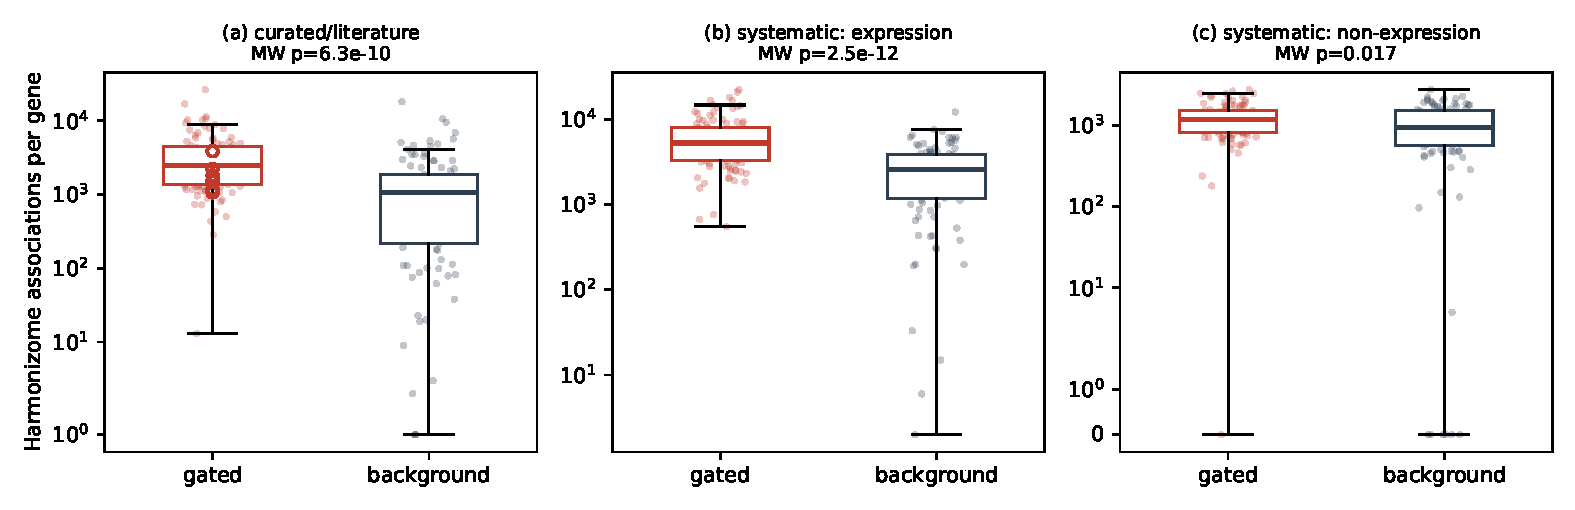
\includegraphics[width=\linewidth]{harmonizome_fig.pdf}
\caption{Harmonizome associations per gene (symlog axis), gated versus
background, in (a) curated/literature, (b) systematic expression and (c)
systematic non-expression datasets. AND-gate antigens are ringed in (a).}
\label{fig:harmonizome}
\end{figure}
